\documentclass{article}
\usepackage{amsfonts}
\usepackage{amsmath}
\usepackage{amsthm}
\usepackage{hyperref}
\usepackage{graphicx}
\usepackage{cleveref}
\usepackage{booktabs}
\usepackage{txfonts}
\usepackage{minted}

\begin{document}
\section{Neural Networks and Deep Learning}
See \url{https://www.deeplearning.ai/} for the course.
\subsection{Introduction}
Machine learning has different applications
\begin{itemize}
\item real estate, online advertising (standard neural networks)
\item image classification (CNN)
\item audio to text, language translation (RNN)
\item position of other cars in autonomous driving (hybrid)
\end{itemize}

Supervised learning uses data consisting of input (x) and desired output (y).
In supervised learning there is structured data (house price and features)
and unstructured data (images, audio, text).

Traditional approaches hit a performance plateau as more and more data becomes available.
Deep learning is facilitated by
\begin{itemize}
\item larger datasets
\item more computational power
\item algorithmic improvements
\end{itemize}

Geoffrey Hinton's advice:
\begin{itemize}
\item read enough so that you start developing intuitions
\item trust your intuitions
\item never stop programming
\end{itemize}

\subsection{Basics of Neural Network programming}
\subsubsection{Binary Classification}
Logistic regression is an algorithm for binary classification (e.g. y=1 (cat) vs y=0 (no cat)).
The training set consists of samples $(x,y)$ with $x\in\mathbb{R}^{n_x}$ and $y\in\{0,1\}$.
The training set is $(x^{(1)},y^{(1)}), (x^{(2)},y^{(2)}), \ldots, (x^{(m)},y^{(m)})$ with $m=m_{train}$ (or $m=m_{test}$ for the test set).
The training data is represented by the matrix
\begin{equation}
  X=\begin{pmatrix}x^{(1)} & x^{(2)} & \cdots & x^{(m)}\end{pmatrix}\in\mathbb{R}^{n_x\times m}
\end{equation}
The labels are
\begin{equation}
  Y=\begin{pmatrix}y^{(1)} & y^{(2)} & \cdots & y^{(m)}\end{pmatrix}\in\mathbb{R}^{1\times m}
\end{equation}

Logistic regression tries to model the probability $\hat{y}=P(y=1|x)$.
The model has the parameters $w\in\mathbb{R}^{n_x}$ and $b\in\mathbb{R}$.
The model is $\hat{y}^{(i)}=\sigma(w^\top x^{(i)}+b)$ using $\sigma(z^{(i)})=\frac{1}{1+e^{-z^{(i)}}}$.
Also see \cref{fig:sigmoid}.
\begin{figure}[htbp]
  \begin{center}
    \includegraphics[width=.5\textwidth]{sigmoid}
    \caption{The sigmoid activation function}
    \label{fig:sigmoid}
  \end{center}
\end{figure}

\subsubsection{Cost function}
The logistic regression \emph{loss function} computes the error for a single training example.
\begin{equation}
  \mathcal{L}(\hat{y},y)=-\big(y\log\hat{y}+(1-y)\log(1-\hat{y})\big)
\end{equation}
with $y\in\{0,1\}$.
The \emph{cost function} is the average of the loss function of the entire training set.
\begin{equation}
  J(w,b)=\frac{1}{m}\sum_{i=1}^m\mathcal{L}(\hat{y}^{(i)},y^{(i)})=
  -\frac{1}{m}\sum_{i=1}^m\big[y^{(i)}\log\hat{y}^{(i)}+(1-y^{(i)})\log(1-\hat{y}^{(i)})\big]
\end{equation}

\subsubsection{Gradient descent}
Gradient descent iteratively minimizes $J(w,b)$ using partial derivatives of $J$.
\begin{equation}
  \begin{split}
    w&\coloneqq w-\alpha\underbrace{\frac{\partial J(w,b)}{\partial w}}_{\eqqcolon dw}\\
    b&\coloneqq b-\alpha\underbrace{\frac{\partial J(w,b)}{\partial b}}_{\eqqcolon db}
  \end{split}
\end{equation}
$\alpha$ is the learning rate.

Derivative chain-rule: $\frac{df(g(x))}{dx}=\frac{df}{dg}\frac{dg}{dx}$.
In the source code $\frac{dJ}{dv}$ is named ``dv'' where $J$ is the final output variable.

In the case of logistic regression with two features $z=w_1x_1+w_2x_2+b$ and $a=\sigma(z)$.
\begin{equation}
  \begin{split}
    \frac{d\mathcal{L}(a,y)}{da}&=-\frac{y}{a}+\frac{1-y}{1-a}\\
    \frac{da}{dz}&=a(1-a)\\
    ``dz''=\frac{d\mathcal{L}}{dz}&=\frac{d\mathcal{L}}{da}\frac{da}{dz}=a-y
  \end{split}
\end{equation}
$\frac{d\mathcal{L}}{dw_1}=``dw_1''=x_1 dz$, $``dw_2''=x_2dz$, and $``db''=dz$.
The update rule for gradient descent then is
\begin{equation}
  \begin{split}
    w_1&\coloneqq w_1-\alpha dw_1\\
    w_2&\coloneqq w_2-\alpha dw_2\\
    b&\coloneqq b-\alpha db\\
  \end{split}
\end{equation}

\subsubsection{Logistic regression on $m$ examples}
Logistic regression over multiple training examples works by simply summing up the derivatives.
\begin{equation}
  \frac{\partial}{\partial w_1}J(w,b)=\frac{1}{m}\sum_{i=1}^m\underbrace{\frac{\partial}{\partial w_1}\mathcal{L}(a^{(i)},y^{(i)})}_{dw_1^{(i)}}
\end{equation}
See \cref{fig:logistic-regression} for more detail.
\begin{figure}
  \begin{center}
    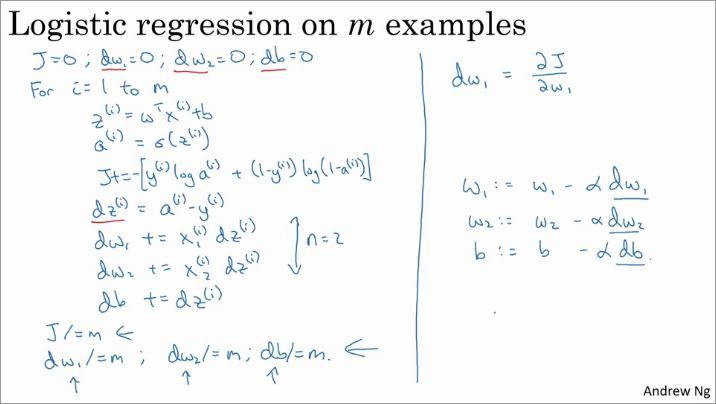
\includegraphics[width=\textwidth]{logistic-regression}
    \caption{Logistic regression on $m$ examples}
    \label{fig:logistic-regression}
  \end{center}
\end{figure}

\subsubsection{Vectorizing Logistic Regression}
\begin{minted}{python}
# Examples for vectorized code
import numpy as np
u = np.dot(A, v)
u = np.exp(v)
np.log(v)
np.maximum(v, o)
v ** 2
\end{minted}

\begin{equation}
  Z=\begin{bmatrix}z^{(1)} & z^{(2)} & \cdots & z^{(m)}\end{bmatrix}=
    w^\top X + \underbrace{\begin{bmatrix}b & b & \cdots & b\end{bmatrix}}_{\in\mathbb{R}^{1\times m}}
\end{equation}

In Python:
\begin{minted}{python}
  Z = np.dot(w.T, x)+b
\end{minted}

\begin{equation}
  A=\begin{bmatrix}a^{(1)} & a^{(2)} & \cdots & a^{(m)}\end{bmatrix}=\sigma(Z)
\end{equation}

\begin{equation}
  dZ=\begin{bmatrix}dz^{(1)} & dz^{(2)} & \cdots & dz^{(m)}\end{bmatrix}
\end{equation}

\begin{equation}
  dZ=A-Y
\end{equation}

\begin{equation}
  db=\frac{1}{m}\sum_{i=1}^m dz^{(i)}
\end{equation}

\begin{minted}{python}
A = sigmoid(np.dot(w.T, X) + b)
cost = -np.sum(Y * np.log(A) + (1 - Y) * np.log(1 - A)) / m
dw = np.dot(X, (A - Y).T) / m
db = np.sum(A - Y) / m
\end{minted}

\begin{equation}
  dw=\frac{1}{m}X dz^\top
\end{equation}

\begin{equation}
  \begin{split}
    w &\coloneqq w-\alpha dw\\
    b &\coloneqq b-\alpha db
  \end{split}
\end{equation}

\subsubsection{Logistic Regression Cost Function}
The two cases
\begin{itemize}
  \item if $y=1$: $p(y|x)=\hat{y}$
  \item if $y=0$: $p(y|x)=1-\hat{y}$
\end{itemize}
can be expressed as one equation: $p(y|x)=\hat{y}^y(1-\hat{y})^{(1-y)}$.
Then
\begin{equation}
  \log p(y|x)=y\log\hat{y}+(1-y)\log(1-\hat{y})
\end{equation}

Overall log-probability to maximise (maximum likelihood)
\begin{equation}
  \log\prod_{i=1}^m p(y^{(i)}|x^{(i)})=\sum_{i=1}^m \underbrace{\log p(y^{(i)}|x^{(i)})}_{-\mathcal{L}(y^{(i)}|x^{(i)})}
\end{equation}
I.e. minimize the negative value
\begin{equation}
  J(w,b)=\frac{1}{m}\sum_{i=1}^m \mathcal{L}(y^{(i)}|x^{(i)})
\end{equation}
which is the cost function.

Interview with Pieter Abbeel on reinforcement learning applied to robotics.

\subsection{One hidden layer Neural Network}
\subsubsection{Neural Network Overview}
\begin{equation}
  \begin{split}a
    z&=w^\top x+b\\
    a&=\sigma(z)\\
    \mathcal{L}(a,y)&=-y\log(a)-(1-y)\log(1-a)
  \end{split}
\end{equation}

In a neural network with one hidden layer we have:
\begin{equation}
  \begin{split}
    z^{[1]}&=W^{[1]}x+b^{[1]}\\
    a^{[1]}&=\sigma(z^{[1]})\\
    z^{[2]}&=W^{[2]}a^{[1]}+b^{[2]}\\
    a^{[2]}&=\sigma(z^{[2]})\\
    \mathcal{L}(a^{[2]},y)&=-y\log(a^{[2]})-(1-y)\log(1-a^{[2]})
  \end{split}
\end{equation}

\subsubsection{Neural Network Representation}
There is
\begin{itemize}
  \item an input layer $a^{[0]}=x$ ($x_1, x_2, \ldots)$
  \item zero, one, or more hidden layer(s) $a^{[l]}$ with $l\in\{1,2,\ldots,L-1\}$
  \item an output layer $\hat{y}=a^{[L]}$
\end{itemize}
Only the input layer is not counted, \emph{e.g.} a 2 layer neural network has 1 hidden layer.
\begin{equation}
  W^{[l]}=
  \begin{pmatrix}
  w^{[l]\top}_1\\
  w^{[l]\top}_2\\
  \vdots
  \end{pmatrix}
\end{equation}

\subsubsection{Vectorizing across multiple examples}
\begin{equation}
  \begin{split}
    x^{(1)}&\to a^{[L](1)}=\hat{y}^{(1)}\\
    x^{(2)}&\to a^{[L](2)}=\hat{y}^{(2)}\\
    &\vdots\\
    x^{(m)}&\to a^{[L](m)}=\hat{y}^{(m)}
  \end{split}
\end{equation}
The computation of multiple training examples is vectorized using
\begin{equation}
  X=\begin{pmatrix}x^{(1)} & x^{(2)} & \cdots & x^{(m)}\end{pmatrix}\in\mathbb{R}^{n_x\times m}
\end{equation}
(by stacking vectors horizontally) as follows
\begin{equation}
  \begin{split}
    Z^{[1]}&=W^{[1]}X+b^{[1]}\\
    A^{[1]}&=\sigma(Z^{[1]})\\
    Z^{[2]}&=W^{[2]}A^{[1]}+b^{[2]}\\
    A^{[2]}&=\sigma(Z^{[2]})
  \end{split}
\end{equation}

\subsubsection{Activation Functions}
\begin{itemize}
  \item $\sigma(z)=\frac{1}{1+e^{-z}}\in[0,1]$
  \item $\tanh z=\frac{e^z-e^{-z}}{e^z+e^{-z}}\in[-1,1]$
  \item $\operatorname{ReLU}(z)=\max(0, z)$
\end{itemize}

The $\tanh$ function generally is better than $\sigma$ because the mean of the output is zero.
One exception is the output layer where inputs between zero and one are desirable.

\subsubsection{Derivatives of Activation Functions}
\begin{equation}
  g(z)=\frac{1}{1+e^{-z}}\to g^\prime(z)=g(z)(1-g(z))
\end{equation}
\begin{equation}
  g(z)=\tanh{z}\to g^\prime(z)=1-\big(g(z)\big)^2
\end{equation}
\begin{equation}
  g(z)=\max(0, z)\to g^\prime(z)=\left\{\begin{array}{ll}0&\mathrm{\ if\ }z<0\\1&\mathrm{\ if\ }z>0\end{array}\right.
\end{equation}

\subsubsection{Gradient descent for neural networks}\label{cha:gradneural}
Forward propagation:
\begin{equation}
  \begin{split}
    Z^{[1]}&=W^{[1]}X+b^{[1]}\\
    A^{[1]}&=g^{[1]}(Z^{[1]})\\
    Z^{[2]}&=W^{[2]}A^{[1]}+b^{[2]}\\
    A^{[2]}&=g^{[2]}(Z^{[2]})=\sigma(Z^{[2]})
  \end{split}
\end{equation}
Backpropagation:
\begin{equation}
  \begin{split}
    dZ^{[2]}&=A^{[2]}-Y\\
    dW^{[2]}&=\frac{1}{m}dZ^{[2]}A^{[1]\top}\\
    db^{[2]}&=\frac{1}{m}\sum_i dZ^{[2](i)}\\
    dZ^{[1]}&=W^{[2]\top}dZ^{[2]}*g^{[1]\prime}(Z^{[1]})\\
    dW^{[1]}&=\frac{1}{m}dZ^{[1]}X\\
    db^{[1]}&=\frac{1}{m}\sum_i dZ^{[1](i)}
  \end{split}
\end{equation}
where ``*'' denotes the elementwise product.

\subsubsection{Random Initialization}
Initializing the weights of a neural network to zero is not sufficient.
The activations will be the same.
By initializing the weights randomly, one can ensure that they are linear independent.
\emph{I.e.} it is necessary to break the symmetry.
Usually the weights are initialised to small random values using a Gaussian random distribution with \emph{e.g.} $\sigma=0.01$.
The bias units can be initialised to zero.

Interview with Ian Goodfellow (Generative Adversarial Neural Networks).
His advice: apply the knowledge to something you are interested in, while learning from the book/online lectures.

\subsection{Deep Neural Networks}
Logistic regression is a ``shallow'' neural network.
A neural network with 5 layers can be called a ``deep'' neural network.
\begin{itemize}
  \item $L$ is the number of layers.
  \item $n^{[l]}$ is the number of units in layer $l$.
  \item $n^{[0]}=n_x$ is the number of input units.
  \item $a^{[l]}=g^{[l]}(z^{[l]})$ is the activation at layer $l$
  \item $a^{[0]}=x$ is the input
  \item $a^{[L]}=\hat{y}$ is the output
  \item $z^{[l]}=W^{[l]}a^{[l-1]}+b^{[l]}$
\end{itemize}

\subsubsection{Forward propagation in a deep network}
\begin{equation}
  \begin{split}
    z^{[1]}&=W^{[1]}x+b^{[1]}\\
    a^{[1]}&=g^{[1]}(z^{[1]})\\
    z^{[2]}&=W^{[2]}a^{[1]}+b^{[2]}\\
    a^{[2]}&=g^{[2]}(z^{[2]})\\
    &\vdots\\
    z^{[L]}&=W^{[L]}a^{[L-1]}+b^{[L]}\\
    \hat{y}&=g^{[L]}(z^{[L]})
  \end{split}
\end{equation}
Using $a^{[0]}=x$ and $a^{[L]}=\hat{y}$ one can write in general:
\begin{equation}
  \begin{split}
    z^{[l]}&=W^{[l]}a^{[l-1]}+b^{[l]}\\
    a^{[l]}&=g^{[l]}(z^{[l]})
  \end{split}
\end{equation}
The vectorized form for a training set (by stacking training examples horizontally):
\begin{equation}
  \begin{split}
    Z^{[l]}&=W^{[l]}A^{[l-1]}+b^{[l]}\\
    A^{[l]}&=g^{[l]}(Z^{[l]})
  \end{split}
\end{equation}

\subsubsection{Getting your matrix dimensions right}
The matrix dimensions are as follows:
\begin{itemize}
  \item $W^{[l]}\in\mathbb{R}^{n^{[l]}\times n^{[l-1]}}$
  \item $b^{[l]}\in\mathbb{R}^{n^{[l]}\times 1}$
  \item $z^{[l]},a^{[l]},dz^{[l]},da^{[l]}\in\mathbb{R}^{n^{[l]}\times 1}$
  \item $Z^{[l]},A^{[l]},dZ^{[l]},dA^{[l]}\in\mathbb{R}^{n^{[l]}\times m}$
\end{itemize}

\subsubsection{Why deep representations}
Using the example of learning $x_1\operatorname{xor}x_2\operatorname{xor}\ldots x_n$ one can show that
it can be represented using a deep neural network with $O(\log n)$ layers and $O(n)$ units.
When using only one hidden layer, $O(2^n)$ units are required.

\subsubsection{Building blocks of of deep neural networks}
See \cref{fig:deepblocks}.
\begin{figure}[htbp]
  \begin{center}
    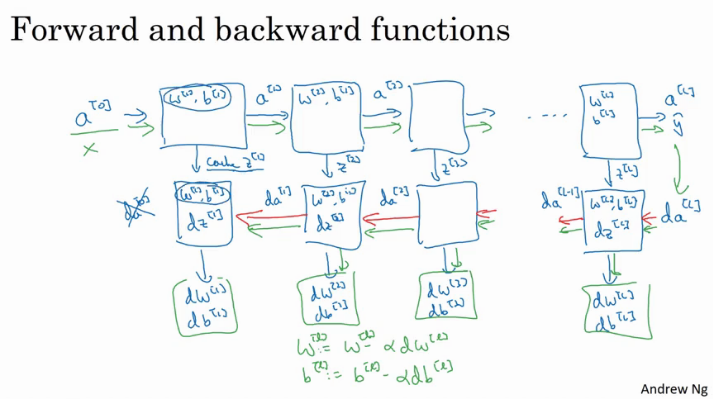
\includegraphics[width=\textwidth]{deepblocks}
    \caption{Building blocks of deep neural network}
    \label{fig:deepblocks}
  \end{center}
\end{figure}

\subsubsection{Forward and Backward Propagation}
\textbf{Forward propagation} for layer $l$:
\begin{itemize}
  \item Input: $a^{[l-1]}$
  \item Output: $a^{[l]}$, cache: $z^{[l]}$
\end{itemize}
The implementation is
\begin{equation}
  \begin{split}
    z^{[l]}&=W^{[l]}a^{[l-1]}+b^{[l]}\\
    a^{[l]}&=g^{[l]}(z^{[l]})
  \end{split}
\end{equation}
The vectorized version simply is
\begin{equation}
  \begin{split}
    Z^{[l]}&=W^{[l]}A^{[l-1]}+b^{[l]}\\
    A^{[l]}&=g^{[l]}(Z^{[l]})
  \end{split}
\end{equation}
where $A^{[0]}=X$.

\textbf{Backward propagation} for layer $l$:
\begin{itemize}
  \item Input: $da^{[l]}$, cached: $z^{[l]}$
  \item Output: $da^{[l-1]}$, $dW^{[l]}$, $db^{[l]}$
\end{itemize}
The implementation is
\begin{equation}
  \begin{split}
    dz^{[l]}&=da^{[l]}*g^{[l]\prime}(z^{[l]})\\
    dW^{[l]}&=dz^{[l]}a^{[l-1]}\\
    db^{[l]}&=dz^{[l]}\\
    da^{[l-1]}&=W^{[l]\top}dz^{[l]}
  \end{split}
\end{equation}
where $da^{[L]}=-\frac{y}{a}+\frac{1-y}{1-a}$.
Note that $dz^{[l]}=W^{[l+1]\top}dz^{[l+1]}*g^{[l]\prime}(z^{[l]})$ similar as in \cref{cha:gradneural}.
The vectorized version is
\begin{equation}
  \begin{split}
    dZ^{[l]}&=dA^{[l]}*g^{[l]\prime}(Z^{[l]})\\
    dW^{[l]}&=\frac{1}{m}dZ^{[l]}A^{[l-1]\top}\\
    db^{[l]}&=\frac{1}{m}\sum_i dZ^{[l](i)}=\frac{1}{m}np.sum(dZ^{[l]}, axis=1,keepdims=True)\\
    dA^{[l-1]}&=W^{[l]\top}dZ^{[l]}
  \end{split}
\end{equation}
where $dA^{[L]}=\sum_{i=1}^m-\frac{y^{(i)}}{a^{(i)}}+\frac{1-y^{(i)}}{1-a^{(i)}}$.

\subsubsection{Parameters vs. Hyperparameters}
$W^{[l]}$ and $b^{[l]}$ with $l\in\{1,2,\ldots,L\}$ are parameters.
Hyperparameters are:
\begin{itemize}
  \item learning rate $\alpha$
  \item number of iterations
  \item number of layers $L$
  \item number of hidden units in each layer
  \item choice of activation function
  \item momentum
  \item minibatch size
  \item regularization parameters
\end{itemize}
Hyperparameters determine the value of the parameters.

\section{Improving Deep Neural Networks: Hyperparameter tuning, Regularisation}
\subsection{Setting up your machine learning application}
\subsubsection{Train / Dev / Test sets}
Split up your data randomly into
\begin{itemize}
  \item training set
  \item hold-out cross-validation set (development set)
  \item test set
\end{itemize}
Traditionally the split was 60\%/20\%/20\% for data sets with 100, 1000, or 10000 samples.
In the modern big data era (1000000 samples) the split can be 98\%/1\%/1\%.

A common problem is a mismatched train/test distribution.
A rule of thumb is to ensure that dev and test set are from the same distribution.

Not having a test set might be okay (if no unbiased estimate is needed).

\subsubsection{Bias/Variance}
The training and dev set error are the main indicator to distinguish between
bias (underfitting) and variance (overfitting) (see \cref{tbl:biasvariance})
\begin{table}[htbp]
  \begin{center}
    \begin{tabular}{crrrr}\toprule
      \textbf{train set performance} &  1\% & 15\% & 15\% & 0.5\%\\
      \textbf{dev set performance}   & 11\% & 16\% & 30\% & 1\%\\\midrule
      & high variance & high bias & both high & both low\\\bottomrule
    \end{tabular}
    \caption{Examples of bias and variance\label{tbl:biasvariance}}
  \end{center}
\end{table}

\subsubsection{Basic Recipe for Machine Learning}
When encountering high \emph{bias}:
\begin{itemize}
  \item bigger network
  \item train longer
  \item neural network architecture search
\end{itemize}
When encountering high \emph{variance}:
\begin{itemize}
  \item more data
  \item regularization
  \item neural network architecture search
\end{itemize}

\subsection{Regularizing your neural network}
\subsubsection{Regularization}
When using logistic regression with $L_2$ regularization one minimizes
\begin{equation}
  J(w,b)=\frac{1}{m}\sum_{i=1}^m\mathcal{L}(\hat{y}^{(i)},y^{(i)})+\frac{\lambda}{2m}||w||_2^2
\end{equation}
where $w\in\mathbb{R}^{n_x}$, $b\in\mathbb{R}$, and $||w||_2^2=\sum_{j=1}^{n_x}w_j^2=w^\top w$
(\emph{i.e.} using the $L_2$ norm).
$\lambda$ is the regularization parameter.

When using a neural network, regularization is implemented as follows
\begin{equation}
  J(W^{[1]},b^{[1]},\ldots,W^{[L]},b^{[L]})=\frac{1}{m}\sum_{i=1}^m\mathcal{L}(\hat{y}^{(i)},y^{(i)})
  +\frac{\lambda}{2m}\sum_{l=1}^L||W^{[l]}||_F^2
\end{equation}
where $||W^{[l]}||_F^2=\sum_{i=1}^{n^{[l]}}\sum_{j=1}^{n^{[l-1]}}(W^{[l]}_{ij})^2$ (Frobenius norm) and
$W^{[l]}\in\mathbb{R}^{n^{[l]}\times n^{[l-1]}}$.
It follows that $dW^{[l]}=(\mathrm{from\ backprop})+\frac{\lambda}{m}W^{[l]}$.
$L_2$ regularization sometimes is also called ``weight decay''.

\subsubsection{Dropout regularization}
Dropout randomly eliminates units from the network during training.
Dropout can be implemented using ``inverted dropout''.
\emph{E.g.} for layer 3 using keep\_prob=0.8.
\begin{minted}{python}
d3 = np.random.rand(a3.shape[0], a3.shape[1]) < keep_prob
\end{minted}
The activations a3 are multiplied with the resulting boolean array.
\begin{minted}{python}
a3 = np.multiply(a3, d3)  # a3 *= d3
a3 /= keep_prob
\end{minted}
Note that a3 is scaled so that the expected value for $Z^{[4]}$ does not change.
When doing backpropagation, dA is multiplied with the same boolean array and scaled with the same factor.
\begin{minted}{python}
da3 = np.multiply(da3, d3)
da3 /= keep_prob
\end{minted}
At test time dropout is \emph{not used}.
keep\_prob can have different values for each layer.

\subsubsection{Why does drop-out work?}
Intuition: Each unit can't rely on any one feature, so have to spread out weights.
The downside of dropout is that the cost function $J$ is not well defined any more.

\subsubsection{Other regularization methods}
\textbf{Data augmentation:}
\begin{itemize}
  \item given images one can flip them horizontally to double the data available
  \item one can crop images or randomly distort or rotate them to synthesize more images
\end{itemize}
\textbf{Early stopping:}
The training and dev set error are plotted.
Usually the dev set error while go down for a while and then eventually increases from there.
One can stop before the dev set error goes up.
The downside of early stopping is that the tasks of minimizing $J$ and not overfitting are coupled
and cannot be worked on independently any more.

\subsection{Setting up your optimization problem}
\subsubsection{Normalizing Inputs}\label{cha:norminputs}
Normalizing the inputs consists of two steps:
\begin{enumerate}
  \item subtract the mean $\mu = \frac{1}{m}\sum_{i=1}^m x^{(i)}$
  \item normalize the variance $\sigma^2=\frac{1}{m}\sum_{i=1}^m(x^{(i)}-\mu)^2$
\end{enumerate}
Note that you should use the same $\mu$ and $\sigma$ for the test set as you use for the training set.
Normalizing the input features improves the symmetry of the cost function and allows you to use a faster learning rate.

\subsubsection{Vanishing/Exploding Gradients}
The slopes in deep networks can get very large or very small.

\subsubsection{Weight Initialization for Deep Networks}
The weights for a single neuron $z=w_1x_1+w_2x_2+\ldots+w_nx_n$ should be initialised with $Var(w_i)=\frac{2}{n}$.
\begin{equation}
  W^{[l]}=np.random.randn(shape)*np.sqrt(\frac{2}{n^{[l-1]}})
\end{equation}
where $n^{[l-1]}$ is the number of inputs for layer $l$.
The optimal variance depends on the activation function.
\begin{itemize}
  \item for $\tanh$ use variance of $\sqrt{\frac{1}{n^{[l-1]}}}$
  \item for ReLU use variance of $\sqrt{\frac{2}{n^{[l-1]}}}$
\end{itemize}
The variance for random initialisation can also be a hyperparameter to optimize.

\subsubsection{Numerical approximation of gradients}
$f^\prime(\theta)$ can be estimated using
$f^\prime(\theta)\approx\frac{f(\theta+\epsilon)-f(\theta-\epsilon)}{2\epsilon}$ where $\epsilon$ is a small value.

\subsubsection{Gradient checking}
\begin{itemize}
  \item Take $W^{[1]},b^{[1]},\ldots,W^{[L]},b^{[L]}$ and reshape into a big vector $\theta$.
  \item Take $dW^{[1]},db^{[1]},\ldots,dW^{[L]},db^{[L]}$ and reshape into a big vector $d\theta$.
  \item For each $i$:
    \begin{itemize}
      \item $d\theta_{approx}[i]=
        \frac{J(\theta_1,\theta_2,\ldots,\theta_i+\epsilon,\ldots)- J(\theta_1,\theta_2,\ldots,\theta_i-\epsilon,\ldots)}{2\epsilon}
        \approx d\theta[i]=\frac{\partial J}{\partial\theta_i}$
    \end{itemize}
  \item Check $\frac{||d\theta_{approx}-d\theta||_2}{||d\theta_{approx}||_2+||d\theta||_2}$ is similar order of magnitude as  $\epsilon$
\end{itemize}
If the gradient check fails, one can investigate which component of $d\theta$ is substantially different to
the corresponding component of $d\theta_{approx}$.
Remember to include the regularization term if regularization is used.
Note that gradient checking does not work with dropout.
One can run gradient checking after initialization and then again after having run training for some time.

Yoshua Bengio: Reinforcement learning, how does a human explore and understand the world?
How does causality and high-level abstractions work?
Implement things yourself. Read ICLR proceedings.

\subsection{Optimization Algorithms}
\subsubsection{Mini-batch gradient descent}
Mini-batch gradient descent is a faster gradient descent algorithm.
Instead of using all $m$ examples, the training set is split up into mini-batches
$(X^{\{1\}},Y^{\{2\}}), (X^{\{2\}},Y^{\{2\}}), \ldots$ which get processed sequentially.
A single pass through the training set is called an ``epoch''.

\subsubsection{Understanding mini-batch gradient descent}
Unlike batch gradient descent, when using mini-batch gradient descent, the cost function $J$ does not decrease monotonically.
\emph{Stochastic gradient descent} uses a mini-batch size of $1$.
In practise one uses a mini-batch size between the to extremes $1$ and $m$.
The reason is that vectorization is still used and the convergence is faster.
\begin{itemize}
  \item if your training set, just use batch gradient descent ($m\le 2000$)
  \item typical mini-batch sizes: $64,128,\ldots,1024$
  \item make sure $(X^{\{t\}},Y^{\{t\}})$ fits into CPU/GPU memory
\end{itemize}
Mini-batch size can be seen as a hyper parameter to optimize.

\subsubsection{Exponentially weighted averages}
One can compute an exponentially weighted average of a sequence $\theta_1,\theta_2,\ldots$
using $v_0=0$ and $v_t=\beta\theta_{t-1}+(1-\beta)\theta_t$.

\subsubsection{Bias correction in exponentially weighted averages}
$v_t=\beta v_{t-1}+(1-\beta)\theta_t$ starts at $0$, \emph{i.e.} is biased initially.
The bias corrected value is $\frac{v_t}{1-\beta^t}$.

\subsubsection{Gradient descent with momentum}
Exponentially weighted averages of the gradient can be used to update the parameters.
This allows you to increase the learning rate.
\begin{equation}
  \begin{split}
    V_{dW}=&\beta V_{dW}+(1-\beta)dW\\
    V_{db}=&\beta V_{db}+(1-\beta)db\\
    W&\coloneqq W-\alpha V_{dW}\\
    b&\coloneqq b-\alpha V_{db}
  \end{split}
\end{equation}
Gradient descent with momentum has the two hyperparameters $\alpha$ and $\beta$.
Typical value for $\beta$ is $0.9$.

\subsubsection{RMSprop}
On iteration $t$:
\begin{itemize}
  \item Compute $dW$, $db$ on current mini-batch
  \item $s_{dW}=\beta_2 s_{dW}+(1-\beta_2)dW^2$ (exponential average of element-wise square)
  \item $s_{db}=\beta_2 s_{db}+(1-\beta_2)db^2$ (exponential average of element-wise square)
  \item $W\coloneqq W-\alpha\frac{dW}{\sqrt{s_{dW}}+\epsilon}$
  \item $b\coloneqq b-\alpha\frac{db}{\sqrt{s_{db}}+\epsilon}$
\end{itemize}
$\epsilon$ is used to prevent division by zero.

\subsubsection{Adam optimization algorithm}
The Adam\footnote{Adaptive moment estimation} optimization algorithm is one of the few optimization algorithms
which work well on a wide range of problems.
The Adam optimization algorithm basically combines gradient descent with momentum and RMSprop.
\begin{itemize}
  \item $V_{dW}=0$, $s_{dW}=0$, $V_{db}=0$, $s_{db}=0$
  \item On iteration $t$:
    \begin{itemize}
      \item compute $dW$, $db$ using current mini-batch
      \item $V_{dW}=\beta_1 V_{dW}+(1-\beta_1)dW$, $V_{db}=\beta_1 V_{db}+(1-\beta_1)db$
      \item $s_{dW}=\beta_2 s_{dW}+(1-\beta_2)dW^2$, $s_{db}=\beta_2 s_{db}+(1-\beta_2)db^2$
      \item $V_{dW}^{corrected}=V_{dW}/(1-\beta_1^t)$, $V_{db}^{corrected}=V_{db}/(1-\beta_1^t)$
      \item $s_{dW}^{corrected}=s_{dW}/(1-\beta_2^t)$, $s_{db}^{corrected}=s_{db}/(1-\beta_2^t)$
      \item $W\coloneqq W-\alpha\frac{V_{dW}^{corrected}}{\sqrt{s_{dW}^{corrected}}+\epsilon}$,
        $b\coloneqq b-\alpha\frac{V_{db}^{corrected}}{\sqrt{s_{db}^{corrected}}+\epsilon}$
    \end{itemize}
\end{itemize}
The hyperparameter $\alpha$ needs to be tuned.
A common choice for $\beta_1$ is $0.9$ (first moment) and for $\beta_2$ is $0.999$ (second moment).
One can use $\epsilon=10^{-8}$.

\subsubsection{Learning rate decay}
One can slowly reduce the learning rate over time to reduce the noise introduced by mini-batches
when approaching the minimum.
\begin{equation}
  \alpha=\frac{1}{1+\mathrm{decay\ rate}*\mathrm{epoch\ num}}\alpha_0
\end{equation}
Other learning rate decay methods are
\begin{itemize}
  \item $\alpha=0.95^{\mathrm{epoch\ num}}\alpha_0$ (exponential decay)
  \item $\alpha=\frac{k}{\sqrt{\mathrm{epoch\ num}}}\alpha_0$ or $\frac{k}{\sqrt{t}}\alpha_0$
\end{itemize}

\subsubsection{The problem of local optima}
High-dimensional spaces rather have saddle points than local minima.
However plateaus can slow down learning.

\subsection{Hyperparameter tuning}
\subsubsection{Tuning process}
\begin{itemize}
  \item $\alpha$
  \item $\beta$
  \item $\beta_1$, $beta_2$, $\epsilon$
  \item \#layers
  \item \#hidden units
  \item learning rate decay
  \item mini-batch size
\end{itemize}
When trying out combinations of hyperparameters, use random values instead of sampling a grid.
This way one tries out more distinct values of each hyperparameter.
Additionally one can use a coarse to fine scheme. \emph{I.e.} sampling more densely where the best results were found.

\subsubsection{Using an appropriate scale to pick hyperparameters}
For number of hidden units and number of layers one can sample a uniform random distribution.
In the case of the learning rate $\alpha$ one uses a logarithmic scale.
\emph{E.g.} $\alpha=10^r$ where $r$ is sampled from a uniform random distribution between $-4$ and $0$.
In a similar fashion one can sample $\beta=1-10^r$ where $r$ is sampled from a uniform random distribution between $-3$ and $-1$.

\subsubsection{Hyperparameter tuning in practice: Pandas vs. Caviar}
Re-test hyperparameters occassionally (after acquiring more data for example).
You can either ``babysit'' (update parameters during training) a single model if a lot of processing is required (Panda approach).
If many models can be trained in parallel, one can simply pick the best one (Caviar approach).

\subsection{Batch Normalization}
\subsubsection{Normalizing activations in a network}
Normalizing inputs speeds up learning (see \cref{cha:norminputs}).
In a similar fashion one can normalize the values $Z^{[l]}$ in each layer $l$.
Given the values $z^{(1)},\ldots,z^{(m)}$ of a layer, one computes
\begin{equation}
  \begin{split}
    \mu&=\frac{1}{m}\sum_i z^{(i)}\\
    \sigma^2&=\frac{1}{m}\sum_i (z^{(i)}-\mu)^2\\
    z^{(i)}_{norm}&=\frac{z^{(i)}-\mu}{\sqrt{\sigma^2+\epsilon}}\\
    \tilde{z}^{(i)}&=\gamma z^{(i)}_{norm}+\beta
  \end{split}
\end{equation}
where $\gamma$ and $\beta$ are learnable parameters of the model.
The values $\tilde{z}^{(i)}$ are then used instead of $z^{(i)}$ for continuing forward propagation.

\subsubsection{Fitting Batch Norm into a neural network}
\begin{equation}
  \begin{split}
    z^{[l]}&=W^{[l]}a^{[l-1]}\\
    \tilde{z}^{[l]}&=\gamma^{[l]}\frac{z^{[l]}-\mu}{\sqrt{\sigma^2+\epsilon}}+\beta^{[l]}\\
    a^{[l]}&=g^{[l]}(\tilde{z}^{[l]})
  \end{split}
\end{equation}
The vector values $\mu$ and $\sigma$ of each layer are computed for the current mini-batch.
Note that $b^{[l]}$ is set to zero because it is made redundant by the vector $\beta^{[l]}$.

\subsubsection{Batch norm at test time}
When testing the neural network, values for $\mu$ and $\sigma^2$ are required.
The values for $\mu$ and $\sigma^2$ can be obtained by computing an exponentially weighted average
of those values at training time.

\subsection{Multi-class classification}
\subsubsection{Softmax regression}
Softmax regression is a generalisation of logistic regression to multiple classes.
\emph{E.g.} recognising four classes cats, dogs, baby chicks, and other.
In this case the output layer has $C=4$ units.
\emph{I.e.} $\hat{y}\in\mathbb{R}^C$.
The softmax activation function are as follows:
\begin{equation}
  \begin{split}
    Z^{[L]}&=W^{[L]}a^{[L-1]}+b^{[L]}\\
    t&=e^{(Z^{[L]})}\\
    a_i^{[L]}&=\frac{t_i}{\sum_{j=1}^C t_i}
  \end{split}
\end{equation}

\subsubsection{Training a softmax classifier}
Note that softmax regression with $C=2$ reduces to logistic regression.
The loss function for softmax regression is
\begin{equation}
  \mathcal{L}(\hat{y},y)=-\sum_{j=1}^C y_j\log\hat{y}_j
\end{equation}
where $y$ always is a basis vector with a single one and the rest zeros.
The cost function is
\begin{equation}
  J(W^{[1]},b^{[1]},\ldots)=\frac{1}{m}\sum_{i=1}^m\mathcal{L}(\hat{y}^{(i)},y^{(i)})
\end{equation}
In a vectorized implementation $Y\in\mathbb{R}^{C\times m}$.

The backpropagation step is (similar as for logistic regression in \cref{cha:gradneural})
\begin{equation}
  \frac{\partial J}{\partial z^{[L]}}=\hat{y}-y
\end{equation}

\subsection{Introduction to programming frameworks}
\subsubsection{Deep learning frameworks}
\begin{itemize}
  \item Caffe/Caffe2
  \item CNTK
  \item DL4J
  \item Keras
  \item Lasagne
  \item mxnet
  \item PaddlePaddle
  \item Tensorflow
  \item Theano
  \item Torch
\end{itemize}
Important criteria when choosing a deep learning framework are
\begin{itemize}
  \item ease of programming (development and deployment)
  \item running speed
  \item truly open (open source with good governance)
\end{itemize}

\subsubsection{Tensorflow}
The example is to minimize
\begin{equation}
  J(w)=w^2-10w+25
\end{equation}
\begin{minted}{python}
import tensorflow as tf
w = tf.Variable(0, dtype=tf.float32)
cost = tf.add(tf.add(w ** 2, tf.multiply(-10, w)), 25)
train = tf.train.GradientDescentOptimizer(0.01).minimize(cost)
init = tf.global_variables_initializer()
session = tf.Session()
session.run(init)
for i in range(1000):
  session.run(train)
print(session.run(w))
\end{minted}
It is only necessary to define the forward propagation.
Tensorflow is able to derive the derivatives necessary for the backward propagation step.
For training data one uses a placeholder. For example
\begin{minted}{python}
x = tf.placeholder(tf.float32, [3, 1])
coefficients = np.array([[1.], [-10.], [25.]])
session.run(train, feed_dict={x: coefficients})
\end{minted}

\section{Structuring Machine Learning Projects}
\subsection{Introduction to ML Strategy}
\subsubsection{Why ML Strategy}
It is important to have a quick and effective way to figure out which of all the ideas are worth pursuing and which you can discard.

\subsubsection{Orthogonalization}
It is important that the different controls of the machine learning system have interpretable effects.
\emph{I.e.} one wants to change one thing at a time.
Things to control in machine learning are
\begin{itemize}
  \item fit training set well on cost function (train bigger network, use better optimization algorithm)
  \item fit dev set well on cost function (regularization, bigger training set)
  \item fit test set well on cost function (bigger dev set)
  \item performs well in real world (change dev set or the cost function)
\end{itemize}
In contrast early stopping simultaneously affects training and dev set performance.

\subsection{Setting up your goal}
\subsubsection{Single number evaluation metric}
It is recommended to setup a single number evaluation metric to measure the performance of your algorithm.
\begin{itemize}
  \item precision: what percentage of the classified examples are correctly classified
  \item recall: what percentage of the available class examples are detected
\end{itemize}
A single number evaluation metric represents the trade-off between precision and recall
(i.e. use F1 score $\frac{2}{\frac{1}{P}+\frac{1}{R}}$ ``harmonic mean'').

\subsubsection{Satisficing and Optimizing metric}
Example: maximize accuracy subject to running time $\le 100ms$.
Then the accuracy is an optimizing metric while the running time is a satisficing metric.
In general you can have one optimizing metric and many satisficing metrics.
Another example is to optimize the accuracy subject to a certain limit on the number of false positives.

\subsubsection{Train/dev/test distributions}
It is important for the training and dev set to come from the same distribution.
The dev set together with the evaluation metric are the target for development of the algorithm.
\textbf{Choose a dev set and test set to reflect data you expect to get in the future and consider important to do well on.}

\subsubsection{Size of the dev and test sets}
The old way of splitting data 60\%/20\%/20\% applies to small test sets ($\le 10000$ samples).
When there is sufficient data (\emph{e.g.} 1000000 samples) then one can split 98\%/1\%/1\%.
Set your test set to be big enough to give high confidence in the overall performance of your system

\subsubsection{When to change dev/test sets and metrics}
Sometimes when trying the algorithm in the real world, one realises that one has to change the evaluation metric.
\emph{E.g.} you can weight some samples in the dev and test set more strongly.
It is important to change the metric to capture your preferences instead of coasting with an old metric.
There are two orthogonal tasks:
\begin{enumerate}
  \item set target, define where you want to aim
  \item do well on this metric
\end{enumerate}
If doing well on your metric + dev/test set does not correspond to doing well on your application, change your metric and/or dev/test set.

\subsection{Comparing to human-level performance}
\subsubsection{Why human-level performance?}
The theoretical limit for the error (Bayes optimal error) of an algorithm generally is not 100\%
(\emph{e.g.} noisy audio, blurry images).
As long as your algorithm performs worse than a human, you can get more labelled data from humans to train your algorithm.
\begin{itemize}
  \item Get labelled data from humans
  \item Gain insights from manual error analysis: Why did a person get this right?
  \item better analysis of bias/variance
\end{itemize}

\subsubsection{Avoidable bias}
Bayes optimal error can only be overcome by overfitting.
Often human level performance is used as an estimate for Bayes optimal error.
In the following example the decision on what to do is different depending on the human level performance
even though training and dev set performance are the same (see \cref{tbl:human}).
\begin{table}[htbp]
  \begin{center}
    \begin{tabular}{r|r|r}
      human level performance     & 1\%  & 7.5\% \\
      training set performance    & 8\%  & 8\%   \\
      development set performance & 10\% & 10\%  \\\hline
      decision & reduce bias & reduce variance
    \end{tabular}
    \caption{Different decision based on human level performance\label{tbl:human}}
  \end{center}
\end{table}
The difference between training set error and Bayes optimal error can be called ``avoidable bias''.

\subsubsection{Understanding human-level performance}
Human-level performance often is used as a proxy for Bayes error.
In this case the best result (\emph{e.g.} by a group of experts) is used.
In other cases human-level performance is used to show that the system has comparable performance to an expert.
In this case the comparative result (\emph{e.g.} single expert) is enough.
As you approach human-level error it becomes harder to know whether you have a bias or variance problem,
because the Bayes optimal error is not known.

\subsubsection{Surpassing human-level performance}
Algorithms surpass humans at
\begin{itemize}
  \item online advertising
  \item product recommendations
  \item logistics (predicting transit time)
  \item loan approvals
\end{itemize}
All this examples are using structured data (\emph{i.e.} these are not natural perception tasks).
Furthermore in these application a large amount of data is available.

\subsubsection{Improving your model performance}
The two fundamental assumptions of supervised learning
\begin{enumerate}
  \item You can fit the training set pretty well.
  \item The training set performance generalizes pretty well to the dev/test set.
\end{enumerate}
Reducing avoidable bias
\begin{itemize}
  \item train bigger model
  \item train longer/use better optimization algorithm
  \item NN architecture/hyperparameters search (\emph{e.g.} RNN, CNN)
\end{itemize}
Reducing variance
\begin{itemize}
  \item more data
  \item regularization (L2, dropout, data augmentation)
  \item NN architecture/hyperparameters search
\end{itemize}

Andrej Karpathy: understand machine learning algorithms from scratch, CS231n lectures.

\subsection{Error Analysis}
\subsubsection{Carrying out error analysis}
Manually examining examples where the algorithm is not performing well can give you insights on what to do next.
\emph{I.e.} get 100 mislabelled dev set examples and analyse what kind of mistakes are most common.
For example
\begin{itemize}
  \item fix pictures of dogs being recognized as cats
  \item fix great cats (lions, panthers, etc.) being misrecognized
  \item improve performance on blurry images
\end{itemize}
This helps to prioritize what class of error to work on.

\subsubsection{Cleaning up incorrectly labelled data}
Deep learning algorithms are quite robust to random errors in the training set.
In contrast systematic errors (\emph{e.g.} white dogs classified as cats) are problematic.
During error analysis one can treat incorrectly labelled examples simply as an other class of error.
When correcting incorrect dev/test set examples
\begin{itemize}
  \item apply same process to your dev and test sets to make sure they continue to come from the same distribution
  \item consider examining examples your algorithm got right as well as ones it got wrong
  \item train and dev/test set data may now come from slightly different distributions
\end{itemize}

\subsubsection{Build your first system quickly, then iterate}
\begin{itemize}
  \item Set up dev/test set and metric
  \item build initial system quickly
  \item use bias/variance analysis \& error analysis to prioritize next steps
\end{itemize}

\subsection{Mismatched training and dev/test set}
\subsubsection{Training and testing on different distributions}
It is important that the dev/test set are representative of the application you care about.
\emph{E.g.} dev/test set with data from mobile application and training set mostly data from web pages.

\subsubsection{Bias and Variance with mismatched data distributions}
If training set and dev set are from different distributions it is necessary to carve out (after random shuffling)
a piece of the training set (a training-dev set) in order to be able to distinguish variance from data mismatch in the dev set.
As before you can use human level error as a proxy for Bayes optimal error to estimate avoidable bias.

\subsubsection{Adressing data mismatch}
\begin{itemize}
  \item Carry out error analysis to try to understand the difference between training and dev set
  \item Make training data more similar, or collect more data similar to dev/test set
\end{itemize}
You can use artificial data synthesis to make the training data more similar to the dev set.
Note that synthesized data can lack in variation and might only create a small subset of the data required
which causes the neural network to overfit.

\subsection{Learning from multiple tasks}
\subsubsection{Transfer learning}
You can replace the last layer of a \emph{pre-trained} network with random weights and then train
(\emph{fine tune}) the network on a different task.
If the new data set is small, you can restrict training to the part of the neural network.
Transfer learning from task A to task B makes sense when
\begin{itemize}
  \item task A and task B have the same input
  \item you have a lot more data for task A than task B
  \item low level features from A could be helpful for learning B
\end{itemize}

\subsubsection{Multi-task learning}
Multi-task learning is to apply one neural network to multiple tasks simultaneously.
\emph{E.g.}
\begin{itemize}
  \item detect pedestrians
  \item detect cars
  \item detect stop signs
  \item detect traffic lights
\end{itemize}
Then the loss is $\frac{1}{m}\sum_{i=1}^m\sum_{j=1}^4\mathcal{L}(\hat{y}^{(i)}_j,y^{(i)}_j)$.
Note that in contrast to softmax regression here one image can have multiple labels.
If the data is incompletely labelled, one can just sum over the defined labels.
Multi-task learning makes sense when
\begin{itemize}
  \item training on a set of tasks that could benefit from having shared lower-level features
  \item usually: amount of data you have for each task is quite similar
  \item can train a big enough neural network to do well on all the tasks
\end{itemize}

\subsection{End-to-end deep learning}
\subsubsection{What is end-to-end deep learning}
End-to-end deep learning replaces a pipeline of multiple stages with a single neural network.
Deep learning requires a large dataset in order to have superior performance.
Otherwise one can only omit no or some stages.
In practise often you don't have enough data for the end-to-end approach.
Often you have more data for each of the sub-tasks.
\emph{E.g.} when detecting faces
\begin{itemize}
  \item detect location of face
  \item compared zoomed face to picture in database
\end{itemize}
An examples where end-to-end deep learning works is machine learning.

\subsubsection{Whether to use end-to-end deep learning}
Pros
\begin{itemize}
  \item let the data speak
  \item less hand-designing of components needed
\end{itemize}
Cons
\begin{itemize}
  \item may need large amount of data
  \item excludes potentially useful hand-designed components
\end{itemize}
Applying end-to-end deep learning
\begin{itemize}
  \item key question: do you have sufficient data to learn a function of the complexity needed to map x to y?
\end{itemize}

Ruslan Salakhutdinov: Unsupervised learning/pretraining using Restricted Boltzmann Machines,
now (with increased computing power available) standard backpropagation works better,
current research is unsupervised learning (variational autoencoders, Generative Adversarial Networks),
try different things and don't be afraid to tackle hard problems, also interesting is deep reinforcement learning.

\section{Convolutional Neural Networks}
\subsection{Foundations of Convolutional Neural Networks}
\subsubsection{Computer Vision}
Computer Vision Problems:
\begin{itemize}
  \item image classification (\emph{e.g.} cat or not cat)
  \item object detection (pose detection, multiple objects)
  \item neural style transfer
\end{itemize}
Deep learning on large images would require are a large number of weights if a fully connected network was used.

\subsubsection{Edge Detection Example}
Edges are detected by convolving with a linear shift-invariant filter, \emph{e.g.} the vertical Prewitt filter
(1 1 1 0 0 0 -1 -1 -1), a vertical Sobel filter (1 2 1 0 0 0 -1 -2 -1), or a Scharr filter
(3 10 3 0 0 0 -3 -10 -3).
Convolution is denoted by $*$.
In Tensorflow convolution can be performed using the function ``tf.nn.conv2d''.
Instead of hand-picking the values of the filter, one can use machine learning to choose the individual weights of each filter.

\subsubsection{Padding}
You can use zero-padding so that the output image has the same size as the input.
Otherwise edge pixels are weighted lower and also the output of a deep neural networks becomes very small.
\begin{itemize}
  \item ``valid'': no padding, output image will be smaller; $p=0$
  \item ``same'': padding so that the output size is the same as the input size; $p=\frac{f-1}{2}$ where $f$ is the filter size
\end{itemize}
The filter size $f$ usually is an odd number.

\subsubsection{Strided Convolutions}
The result of the convolution can be subsampled by applying a stride larger than $1$.
The size of the output is $\lfloor\frac{n+2p-f}{s}+1\rfloor$.
Note that in machine learning convolution is actually a cross-correlation.
Convolution is sometimes preferred in signal processing because it is an associative operation.

\subsubsection{Convolutions over Volumes}
An RGB image with $6\times 6\times 3$ elements gets convolved with a $3\times 3\times 3$ filter.
The output is a $4\times 4$ image.
When using multiple filters, the output will be three-dimensional (will have multiple channels).

\subsubsection{One Layer of a Convolutional Network}
A convolutional layer adds a bias unit for each filter followed by the ReLU activation function.
\emph{I.e.} a $3\times 3\times 3$ filter has $3^3+1=28$ parameters.
If layer $l$ is a convolutional layer:
\begin{itemize}
  \item $f^{[l]}$ is the filter size
  \item $p^{[l]}$ is the padding
  \item $s^{[l]}$ is the stride
  \item $n^{[l]}_C$ is the number of filters
\end{itemize}
The input is of size $n^{[l-1]}_H\times n^{[l-1]}_W\times n^{[l-1]}_C$.
The output and the activations are of size $n^{[l]}_H\times n^{[l]}_W\times n^{[l]}_C$.
Each filter is of size $f^{[l]}\times f^{[l]}\times n^{[l-1]}_C$.
\begin{equation}
  \begin{split}
    n^{[l]}_H&=\lfloor\frac{n^{[l-1]}_H+2p^{[l]}-f^{[l]}}{s^{[l]}}+1\rfloor\\
    n^{[l]}_W&=\lfloor\frac{n^{[l-1]}_W+2p^{[l]}-f^{[l]}}{s^{[l]}}+1\rfloor
  \end{split}
\end{equation}
When using batch gradient descent the activations $A^{[l]}$ will have size
$m\times n^{[l]}_H\times n^{[l]}_W\times n^{[l]}_C$.
The weights will have size $f^{[l]}\times f^{[l]}\times n^{[l-1]}_C\times n^{[l]}_C$.
The biases will have size $n^{[l]}_C$.

\subsubsection{Simple Convolutional Network Example}
As you go deeper into a network the height and width decreases while the number of channels increases.
Finally a fully connected logistic or softmax layer uses the stacked output of the last convolutional layer.
A convolutional neural network usually has the following layers
\begin{itemize}
  \item convolution (CONV)
  \item pooling (POOL)
  \item fully connected (FC)
\end{itemize}

\subsubsection{Pooling Layers}
Max-pooling takes the biggest number in each $2\times 2$ region ($f=s=2$).
Max-pooling does not have any parameters to learn.
Usually the channels are not reduced when doing max-pooling.
One can also use average pooling (less common).
The hyperparameters for pooling are $f$ (filter size) and $s$ (stride).
Max pooling usually does not use any padding.
If the input is of size $n_H\times n_W\times n_C$, the output is of size
$\lfloor\frac{n_H-f}{s}+1\rfloor\times\lfloor\frac{n_W-f}{s}+1\rfloor\times n_C$.

\subsubsection{CNN Example}
Often convolutional and max-pooling are seen as one layer (because the pooling layer has no weights).
Also see \cref{tbl:cnnexample}.
\begin{table}
  \begin{tabular}{c|crr}\toprule
    & activation shape & activation size & \#parameters\\\midrule
    input:           & (32, 32,  3) & 3072 &     0 \\
    CONV1 (f=5, s=1) & (28, 28,  8) & 6272 &   608 \\
    POOL1            & (14, 14,  8) & 1568 &     0 \\
    CONV2 (f=5, s=1) & (10, 10, 16) & 1600 &  3216 \\
    POOL2            & (5, 5, 16)   &  400 &     0 \\
    FC3              & (120, 1)     &  120 & 48120 \\
    FC4              & (84, 1)      &   84 & 10164 \\
    Softmax          & (10, 1)      &   10 &   850 \\\bottomrule
  \end{tabular}
  \caption{Example CNN\label{tbl:cnnexample}}
\end{table}

\subsubsection{Why Convolutions?}
The two advantages are
\begin{itemize}
  \item parameter sharing: a feature detector that's usefil in one part of the image is probably useful in another part of the image
  \item sparsity of connections: in each layer, each output value depends only on a small number of inputs
\end{itemize}

\subsection{Deep convolutional models: case studies}
\subsubsection{Why look at case studies?}
A good way to gain intuition about convolutional neural networks is to read/see other examples of effective conv nets.
Some classic networks are:
\begin{itemize}
  \item LeNet-5
  \item AlexNet
  \item VGG
\end{itemize}
More recent networks are
\begin{itemize}
  \item ResNet
  \item Inception
\end{itemize}

\subsubsection{Classic Networks}
\emph{LeCun et al., 1998, Gradient-based learning applied to document recognition}:
LeNet-5 classifies handwritten digits (MNIST) of size $32\times 32\times 1$ (gray scale).
LeNet-5 uses $5\times 5$ filters, average pooling, sigmoid and tanh activation functions,
and conv layers with increasing number of channels.
The final two layers are fully connected layers.
Modern networks rather use max-pooling and ReLU activation functions.
LeNet-5 has about 60,000 parameters.

\emph{Krizhevsky et al., 2012, ImageNet classification with deep convolutional neural networks}:
AlexNet is named after Alex Krizhevsky.
The input size is $227\times 227\times 3$.
It uses $11\times 11$ filters with a stride of $4$, later a $5\times 5$ filter with padding and stride $1$.
Max-pooling uses $3\times 3$ filters and a stride of $2$ in each case.
AlexNet uses the ReLU activation function.
AlexNet as about 160,000,000 parameters and was implemented using multiple GPUs.
Local Response Normalization is used (but has not become popular).

\emph{Simonyan \& Zisserman 2015: Very deep convolutional networks for large-scale image recognition}:
The VGG-16 network just uses $3\times 3$ convolution filters using stride $1$ and same padding.
Max-pooling always uses $2\times 2$ filters with a stride of $2$.
Multiple convolutional layers are used before max-pooling.
The number of channels increases by a factor of $2$ with each group of convolutional layers.
Finally there are two fully connected layers.
Altogether there are $16$ layers.
The network has about 138,000,000 parameters.

\subsubsection{ResNets}
When using deeper networks the training error eventually goes up again.
Also deep networks are difficult to train because of vanishing/exploding gradient types of problems.
Residual networks (ResNets) use skip connections to take activations to another layer much deeper in the neural network.
A residual block uses a skip connection as follows
\begin{equation}
  \begin{split}
    z^{[l+1]}&=W^{[l+1]}a^{[l]}+b^{[l+1]}\\
    a^{[l+1]}&=g(z^{[l+1]})\\
    z^{[l+2]}&=W^{[l+2]}a^{[l+1]}+b^{[l+2]}\\
    a^{[l+2]}&=g(z^{[l+2]}a^{[l]})
  \end{split}
\end{equation}
Also see \emph{He et al., 2015, Deep residual networks for image recognition}.
A neural network with $L$ layers can be converted to a network with $L/2$ residual blocks.

\subsubsection{Why ResNets Work}
If the weight $W^{[l+1]}$ and the bias $b^{[l+1]}$ in a residual block are zero and the ReLU activation function is used,
the residual block outputs $a^{[l]}$, \emph{i.e.} becomes the identity function.
It is easy for a residual block to learn the identity function.
Note that $z^{[l+2]}$ and $a^{[l]}$ need to have the same dimension.
If not, an adapter matrix $W_s$ is used so that $W_s a^{[l]}$ has the same dimension as $z^{[l+2]}$.
$W_s$ can be a diagonal matrix performing zero-padding or it can be learned.

\subsubsection{Network in Network and 1x1 Convolutions}
\emph{Lin et al., 2013, Network in network}:
A 1x1 convolution with a different value for each channel and a different filter for each output layer
is like defining a fully connected network for every pixel (each having multiple channels).
A network in network can be used to reduce the number of channels.
The filter size is $1\times 1\times n^{[l-1]}_C\times n^{[l]}_C$.

\subsubsection{Inception Network Motivation}
\emph{Szegedy et al., 2014, Going deeper with convolutions}:
One can perform different convolutions with different filter sizes as well as max-pooling and stack the output channels
(the width and height of the outputs must be the same).
To reduce the computational cost, one can use a ``bottleneck layer'' ($1\times 1$ convolution) to first shrink the number of channels.

\subsubsection{Inception Network}
\Cref{fig:inception} shows a module of the Inception network.
\begin{figure}
  \begin{center}
    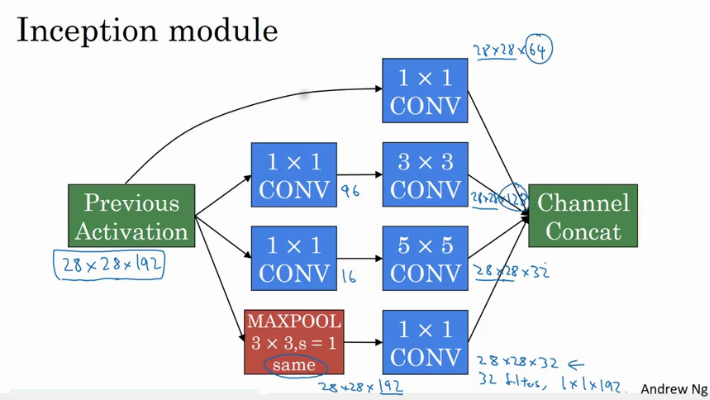
\includegraphics[width=\textwidth]{inception}
    \caption{Inception module}
    \label{fig:inception}
  \end{center}
\end{figure}
The Inception network uses many Inception blocks.
Also there are outputs (side-branches) in the middle of the network which are used to predict the output.
This appears to have a regularizing effect and helps to prevent this network from overfitting.

\subsection{Practical advices for using ConvNets}
\subsubsection{Using Open-Source Implementations}
Even after reading the paper it can be difficult to reproduce results published by another researcher.
Often researchers publish their implementation on Github.

\subsubsection{Transfer Learning}
Rather than training from scratch using random initialization
one can use transfer learning to transfer knowledge from one of the large public datasets.
One initializes the network using the weights from the public network.
Then one can freeze no part, part, or all but the last layer (depending on how much data you have) of the network and train the rest.
To speed up training even more one can precompute the responses of the frozen network for the training set.

\subsubsection{Data Augmentation}
Different data augmentation methods are
\begin{itemize}
  \item mirroring an image
  \item random cropping an image
  \item rotation, shearing, local warping
  \item random color shifting (\emph{e.g.} add RGB(20, -20, 20) to the image), PCA color augmentation
\end{itemize}
In practise often data augmentation and training run in parallel.
The data augmentation parameters are hyperparameters to optimize.

\subsubsection{State of Computer Vision}
There is (relative to the task) little data available for object detection.
There is (relative to the task) lots of data available for speech recognition.
When lots of data is available, one can use simpler algorithms with less hand-engineering.
\emph{I.e.} there are two sources of knowledge
\begin{itemize}
  \item labeled data
  \item hand engineered features/network architecture/other components/transfer learning
\end{itemize}
Tips for doing well on benchmarks/winning competitions
\begin{itemize}
  \item ensembling (train several networks independently and average their outputs)
  \item multi-crop at test time (run classifier on multiple versions of test images and average results)
\end{itemize}

\subsection{Detection algorithms}
\subsubsection{Object Localization}\label{cha:localize}
There are three different algorithms:
\begin{itemize}
  \item image classification: just classify the object
  \item classification with localization: classify and localize object in a picture
  \item detection: classify and localize multiple objects in a picture
\end{itemize}
When doing classification with localization one can use additional outputs $b_x, b_y, b_h, b_w\in[0,1]$ which define a bounding box
with midpoint $(b_x,b_y)$ and bounding box width $b_w$ and height $b_h$.
The output is
\begin{equation}
  y=\begin{pmatrix}p_c\\b_x\\b_y\\b_h\\b_w\\c_1\\c_2\\c_3\end{pmatrix}
\end{equation}
Where $p_c$ decides whether there is an object at all and $c_1,c_2,c_3$ are $1$ if the object belongs to the given class (\emph{e.g.} pedestrian, car, or motorcycle).
Mote that here we assume that there is at most one object shown in the picture.
When $p_c$ is $0$, the other parts of the label are ``?'' (don't care).
One can use a log-likelihood loss for the class labels, square error for the bounding box parameters,
and logistic regression loss for $p_c$.

\subsubsection{Landmark Detection}
One can learn landmark coordinates (\emph{e.g.} corners of left and right eye, or multiple keypoints on a face, pose of a person).
The network then would output $l_{1x},l_{1y},l_{2x},l_{2y},\ldots$.
The coordinates can for example be used for augmented reality.

\subsubsection{Object Detection}
First a neural network is trained to classify tightly cropped images to whether a car is shown in the image or not.
The conv net then is used with a sliding window to exhaustively search the image.
The process is repeated for different window sizes.
This algorithm is called ``sliding windows detection''.

\subsubsection{Convolutional Implementation of Sliding Windows}
\emph{Sermanet et al., 2014, OverFeat: Integrated recognition, localization and detection using convolutional networks}:
One can turn a fully connected layers into a $1\times 1$ convolutional layers (see \cref{fig:convslide}).
Running the same algorithm on the full image instead of the slidding window, one obtains the results for all window positions
while reusing a lot of the computation which is identical between different overlapping slidding windows.
\begin{figure}
  \begin{center}
    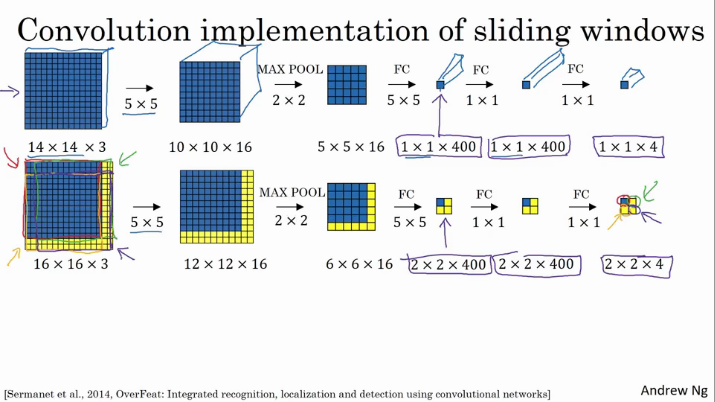
\includegraphics[width=\textwidth]{convslide}
    \caption{Implementing sliding window using $1\times 1$ convolutional layers}
    \label{fig:convslide}
  \end{center}
\end{figure}

\subsubsection{Bounding Box Predictions}
The You Only Look Once (YOLO) algorithm divides up the image into a grid (\emph{e.g.} $19\times 19$).
The training label for an image for example is a $19\times 19\times 8$ (where $8$ is as in \cref{cha:localize}).
Each grid cell can output a bounding box and object class (or no object).
The bounding box coordinates are specified relative to the cell size.
Note that $b_w$ and $b_h$ can be bigger than one.

\section{Sequence Models}

\end{document}
